\documentclass[11pt]{article}
\usepackage[utf8]{inputenc}
\usepackage[T1]{fontenc}
\usepackage{geometry}
\usepackage{hyperref}
\usepackage{graphicx}
\usepackage{longtable}
\usepackage{array}

\usepackage{float}

\geometry{margin=1in}


\newcolumntype{L}[1]{>{\raggedright\arraybackslash}p{#1}}

\title{SRSML24: STM Machine Learning Module}
\author{Steven R. Schofield}
\date{\today}

\begin{document}

\maketitle

\section*{Overview}
This module provides tools for machine learning analysis of scanning tunnelling microscopy (STM) data, including autoencoder models, clustering tools, and STM-specific preprocessing.

\section*{Getting the Code}
Clone the repository from GitHub:

\begin{verbatim}
git clone https://github.com/srschofield/SRSML24.git
\end{verbatim}

\section*{Installation}
It is recommended to create a clean Python environment using \texttt{conda}. The following steps assume you are working on a macOS system with Apple Silicon:

\begin{verbatim}
# create and activate environment
conda create --name srsml24 python=3.8 -y
conda activate srsml24

# install packages
pip install -r requirements-macos.txt
\end{verbatim}

\subsection*{Known Working Configuration}
This module has been tested and is known to work with the following configuration on macOS 15.0.1 (Apple Silicon, M3 Pro chip):
\begin{table}[H]
\centering
\begin{tabular}{ll}
\hline
\textbf{Package} & \textbf{Version} \\
\hline
\texttt{python} & 3.8 \\
\texttt{tensorflow-macos} & 2.13.0 \\
\texttt{tensorflow-metal} & 1.0.1 \\
\texttt{numpy} & 1.24.3 \\
\texttt{pandas} & 2.0.3 \\
\texttt{matplotlib} & 3.7.5 \\
\texttt{scikit-learn} & 1.3.2 \\
\texttt{scipy} & 1.10.1 \\
\texttt{opencv-python} & 4.11.0.86 \\
\texttt{Pillow} & 10.4.0 \\
\texttt{joblib} & 1.4.2 \\
\texttt{jupyter} & 1.1.1 \\
\texttt{ipykernel} & 6.29.5 \\
\texttt{keras-core} & 0.1.5 \\
\texttt{spiepy} & 0.2.1 \\
\texttt{access2thematrix} & 0.4.4 \\
\hline
\end{tabular}
\caption{Verified package versions for macOS (Apple Silicon) environment}
\end{table}


These packages can be installed using the \texttt{requirements-macos.txt} file. The Python version is critical: other versions may cause compatibility issues with TensorFlow or other packages on Apple Silicon.

\section*{Python Files}
\begin{itemize}
  \item \texttt{data\_prep.py} – Functions for data preparation, including slicing STM images into windows and saving them in efficient formats.
  \item \texttt{model.py} – Defines convolutional autoencoder and UNET-style models.
  \item \texttt{utils.py} – Utility functions for loading/saving models, feature arrays, and results.
\end{itemize}

\section*{License}
This work is licensed under the \href{https://creativecommons.org/licenses/by-nc-sa/4.0/}{Creative Commons Attribution-NonCommercial-ShareAlike 4.0 International License (CC BY-NC-SA 4.0)}. You may share and adapt the material for non-commercial purposes, provided that appropriate credit is given and any derivatives are licensed under identical terms.

\pagebreak
\section*{Parameter Summary}

\begin{longtable}{L{0.3\textwidth} L{0.65\textwidth}}
\textbf{Parameter} & \textbf{Description} \\
\hline
\endfirsthead

\textbf{Parameter} & \textbf{Description} \\
\hline
\endhead

\multicolumn{2}{l}{\textbf{General}} \\
\texttt{job\_name} & Label for the run, it will be the folder name for output. \\
\texttt{verbose} & If \texttt{True}, enables more detailed print output. \\

\hline
\multicolumn{2}{l}{\textbf{Matrix data file processing}} \\ 
\texttt{flatten\_method} & Method used to flatten STM images before analysis. Options are `none', `iterate\_mask', `poly\_xy'.\\
\texttt{pixel\_density} & All images will be converted to this pixel density (px/nm). \\
\texttt{pixel\_ratio} & Images that have ratio of fast/slow scan direction less than this will be discared. Setting to 1 means only complete (square) images are kept.\\
\texttt{data\_scaling} & Multiplicative factor for z-height data. Setting to 1.e9 means that the range 0--1 (used for training) corresponds to 1 nm.\\

\hline
\multicolumn{2}{l}{\textbf{Window generation}} \\ 
\texttt{window\_size} & Side length of square image windows (in pixels). \\
\texttt{window\_pitch} & Spacing between adjacent windows during tiling. \\

\hline
\multicolumn{2}{l}{\textbf{Data saving}} \\

\multicolumn{2}{l}{(Should remain defaults but options can be useful for examining data manually.)}\\
\texttt{save\_windows} & If \texttt{True}, saves image windows as \texttt{.npy} files (True).\\
\texttt{together} & If \texttt{True}, saves windows per image in a single file (True). \\
\texttt{save\_jpg} & If \texttt{True}, saves full STM images as JPGs (False).\\ 
\texttt{collate} & If \texttt{True}, flattens directory structure into one folder. (False). \\
\texttt{save\_window\_jpgs} & If \texttt{True}, saves image windows as JPGs. (False)\\

\hline
\multicolumn{2}{l}{\textbf{Autoencoder}} \\ 
\texttt{model\_name} & Label used to save and load the trained autoencoder model. \\
\texttt{batch\_size} & Number of windows per training batch. \\
\texttt{buffer\_size} & Size of shuffle buffer. \\
\texttt{learning\_rate} & Learning rate for the optimizer. \\
\texttt{epochs} & Number of training epochs. \\

\hline
\multicolumn{2}{l}{\textbf{Clustering}} \\ 
\texttt{cluster\_model\_name} & Name used when saving the clustering model. \\
\texttt{cluster\_batch\_size} & Number of latent vectors per clustering batch. \\
\texttt{cluster\_buffer\_size} & Size of buffer for clustering shuffle. \\
\texttt{num\_clusters} & Number of clusters to form using KMeans. \\
\texttt{n\_init} & Number of initializations for KMeans. \\
\texttt{max\_iter} & Max iterations for KMeans convergence. \\
\texttt{reassignment\_ratio} & Fraction of centroids reassigned each step. \\

\hline
\multicolumn{2}{l}{\textbf{Image prediction}} \\ 
\texttt{predict\_window\_pitch} & Window spacing during prediction step. \\
\texttt{mtrx\_train\_data\_limit} & Max number of training MTRX files to use. \\
\texttt{mtrx\_test\_data\_limit} & Max number of validation MTRX files to use. \\
\texttt{train\_data\_limit} & Limit on number of training windows. \\
\texttt{test\_data\_limit} & Limit on number of validation windows. \\
\end{longtable}

\pagebreak

\section*{Step 1: Converting MATRIX STM Data Files}

The initial step in utilizing the SRSML24 module involves converting raw STM data files from the Scienta Omicron MATRIX format into a standardized format suitable for machine learning analysis. This is accomplished using the \texttt{process\_mtrx\_files} function.

\subsection*{Function Overview}

\texttt{process\_mtrx\_files(mtrx\_paths, save\_data\_path, **kwargs)} is designed to batch process a list of MATRIX (\texttt{.mtrx}) files, performing the following operations:

\begin{itemize}
  \item \textbf{Loading Data:} Reads each \texttt{.mtrx} file and extracts image data along with associated metadata.
  \item \textbf{Preprocessing:} Applies flattening methods to correct for background variations and rescales images to a consistent pixel density.
  \item \textbf{Window Extraction:} Divides images into smaller windows of specified size and pitch, facilitating training of machine learning models.
  \item \textbf{Saving Outputs:} Stores processed windows and optional JPEG representations in a structured directory hierarchy under \texttt{save\_data\_path}.
\end{itemize}

This function ensures that STM data is preprocessed consistently, facilitating reliable training and evaluation of machine learning models within the SRSML24 framework. It will create a new directory called ``windows'' and subfolders under that with the names corresponding to the folders the matrix data was stored in (e.g., ``training'' or ``testing''). Unless the ``collate'' variable is set, the windowed data will retain the full directory structure (dates, days, etc) of the matrix data. The individual windows for a given folder of matrix data are all stored within a single .npy file, rather than separate .npy files for each window, since this is much more efficient for data saving and retrieving. Two text files are also saved, one has the meta data (STM bias voltage, current, etc.). The other has the coordinates for each window in the dataset. This is useful since these are not uniform at two edges of the original image for the general case where the full image is not perfectly divided by the dimensions of the individual windows. 

\begin{figure}[H]
\centering
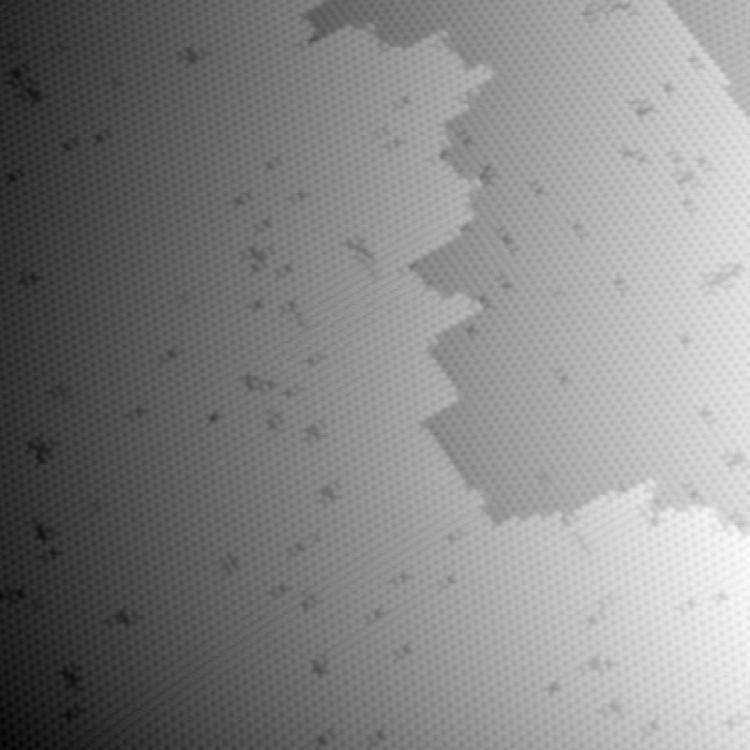
\includegraphics[width=0.4\textwidth]{figs/default_2011Jan07-144939_STM-STM_Spectroscopy--1_1_BD_none}
\hspace{1em}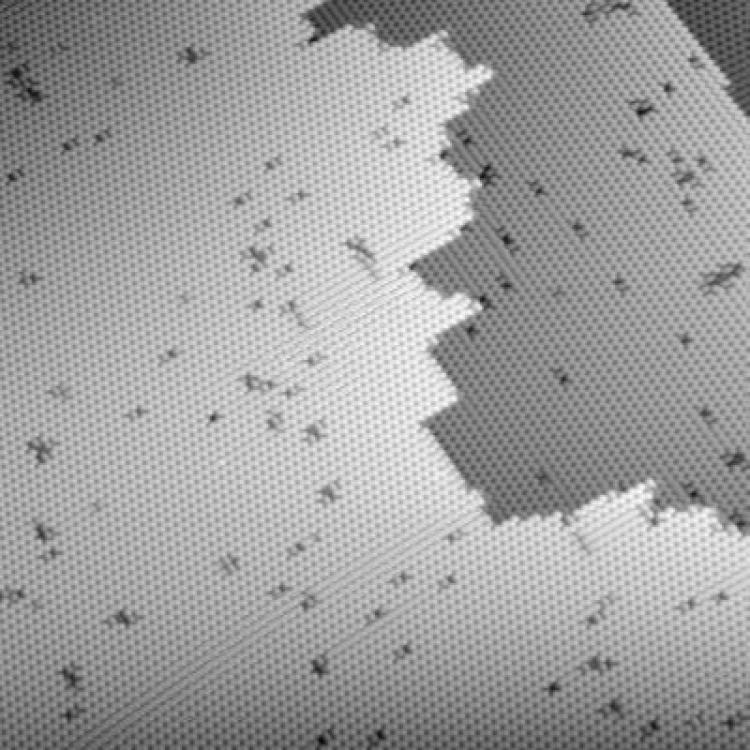
\includegraphics[width=0.4\textwidth]{figs/default_2011Jan07-144939_STM-STM_Spectroscopy--1_1_BD_poly_xy}
\caption{Typical scanning tunnelling microscopy (STM) image. (Left) raw data. (Right) After poly\_xy background subtraction.}
\label{fig:stm}
\end{figure}

\begin{figure}[H]
\centering
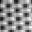
\includegraphics[width=0.07\textwidth]{figs/default_2011Jan07-144939_STM-STM_Spectroscopy--1_1_BD_00032}
\hspace{0.2em}
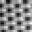
\includegraphics[width=0.07\textwidth]{figs/default_2011Jan07-144939_STM-STM_Spectroscopy--1_1_BD_00033}
\hspace{0.2em}
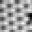
\includegraphics[width=0.07\textwidth]{figs/default_2011Jan07-144939_STM-STM_Spectroscopy--1_1_BD_00034}
\hspace{0.2em}
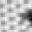
\includegraphics[width=0.07\textwidth]{figs/default_2011Jan07-144939_STM-STM_Spectroscopy--1_1_BD_00035}
\hspace{0.2em}
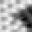
\includegraphics[width=0.07\textwidth]{figs/default_2011Jan07-144939_STM-STM_Spectroscopy--1_1_BD_00036}
\hspace{0.2em}
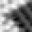
\includegraphics[width=0.07\textwidth]{figs/default_2011Jan07-144939_STM-STM_Spectroscopy--1_1_BD_00037}
\hspace{0.2em}
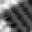
\includegraphics[width=0.07\textwidth]{figs/default_2011Jan07-144939_STM-STM_Spectroscopy--1_1_BD_00038}
\hspace{0.2em}
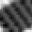
\includegraphics[width=0.07\textwidth]{figs/default_2011Jan07-144939_STM-STM_Spectroscopy--1_1_BD_00039}
\hspace{0.2em}
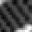
\includegraphics[width=0.07\textwidth]{figs/default_2011Jan07-144939_STM-STM_Spectroscopy--1_1_BD_00040}
\hspace{0.2em}
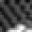
\includegraphics[width=0.07\textwidth]{figs/default_2011Jan07-144939_STM-STM_Spectroscopy--1_1_BD_00041}
\hspace{0.2em}
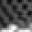
\includegraphics[width=0.07\textwidth]{figs/default_2011Jan07-144939_STM-STM_Spectroscopy--1_1_BD_00042}
\caption{A sequence of $30\times30$ pixel windows extracted from the STM image in Fig.~\ref{fig:stm} with an 8 pixel pitch.}
\end{figure}

\section*{Step 2: Preparing Datasets and Training the Autoencoder}

With windowed STM data in place, the next stage is to set up efficient TensorFlow data pipelines and train a convolutional autoencoder. This step handles the full model lifecycle, from data loading and batching to model training and saving the model and training history. These tools are provided by \texttt{model.py}, which we import as \texttt{m}, i.e., \texttt{import SRSML24.model as m}.

\subsection*{Preparing Datasets with \texttt{tf.data}}

To begin, window data stored as \texttt{.npy} files in \texttt{windows\_train\_path} and \texttt{windows\_test\_path} are listed. If it possible to choose a truncated subset of this list, e.g., to train on less data while optimising; this is done by setting the \texttt{train\_data\_limit} and \texttt{test\_data\_limit} parameters. These files are then loaded into TensorFlow \texttt{Dataset} objects for training and validation.

The function \texttt{m.create\_tf\_dataset\_batched(file\_paths, batch\_size, buffer\_size, window\_size, is\_autoencoder, shuffle)} constructs a pipeline that:

\begin{itemize}
  \item \textbf{Loads image batches:} Reads window data from \texttt{.npy} files located at the specified paths.
  \item \textbf{Shuffles window order:} When \texttt{shuffle=True}, randomizes input order to enhance model generalization.
  \item \textbf{Batches the data:} Groups windows into batches of size \texttt{batch\_size}.
  \item \textbf{Prefetches data:} Uses \texttt{prefetch(buffer\_size)} to improve throughput by overlapping data preparation with model training.
  \item \textbf{Pairs inputs and targets:} For autoencoder training, each window is used as both the input and target.
\end{itemize}

\subsection*{Model Building and Training}

Once the datasets are ready, the autoencoder can be constructed, compiled, and trained using the following workflow:

\begin{itemize}
  \item \textbf{Model instantiation:} 
    \begin{itemize}
      \item Use \texttt{m.build\_autoencoder(window\_size, model\_name)} to define the encoder–decoder architecture.
      \item Call \texttt{model.summary()} to inspect the model structure.
    \end{itemize}
  \item \textbf{Optimizer selection:}
    \begin{itemize}
      \item On Apple Silicon/macOS systems, use \texttt{tf.keras.optimizers.legacy.RMSprop} for TensorFlow-metal compatibility.
      \item On other systems, use the standard \texttt{tf.keras.optimizers.RMSprop}.
    \end{itemize}
  \item \textbf{Compilation:} Compile the model with:
    \begin{itemize}
      \item \texttt{loss='mean\_squared\_error'}
      \item Metrics: \texttt{['mse', 'mae']}
      \item Learning rate: from the \texttt{learning\_rate} parameter.
    \end{itemize}
  \item \textbf{Training:} Fit the model using:
    \begin{itemize}
      \item \texttt{train\_dataset} with \texttt{shuffle=True}
      \item \texttt{validation\_data=test\_dataset}
      \item The number of \texttt{epochs} and \texttt{verbose=1}
    \end{itemize}
  \item \textbf{Saving outputs and diagnostics:}
    \begin{itemize}
      \item Save the trained model using \texttt{m.save\_model(..., model\_train\_time)}.
      \item Record training start/end times with \texttt{dp.current\_datetime()} and \texttt{dp.elapsed\_time()}.
      \item Persist the training history with \texttt{m.save\_history(...)}.
      \item Plot performance metrics via \texttt{m.plot\_history\_from\_file(...)}.
    \end{itemize}
\end{itemize}

This produces a trained autoencoder model along with detailed training logs and performance plots, ready for use in clustering or anomaly detection tasks.


\end{document}
